\chapter{Task execution}
In its most basic implementation, sensors and actuators can be directly tied to each other, removing the need for computation. Such robots are purely reactive, thereby missing the ability to ``think'' or plan. In order to achieve more complex behavior, memory and state are needed to switch between different controllers and algorithms.

This chapter introduces these basic principles as well as their implementation, starting with basic reactive controllers (Section \ref{sec:braitenberg}), then introduces more advanced concepts that let the robot make basic ``if'' \ldots ``then'' decisions using ``Finite State Machines'' (FSM) in Sections \ref{sec:fsm} and \ref{sec:stateflow}, and finally introduces advanced concepts such as ``behavior trees'' and semantic planning in Sections \ref{sec:behaviortrees} and \ref{sec:strips}.

\section{Reactive control}\label{sec:braitenberg}
A large variety of robotic behaviors can be accomplished by directly connecting sensor input to actuator output. These behaviors can even be accomplished without a computer, instead using analog electronics that provide appropriate conditioning. Simple autonomous robots using this concept have been demonstrated as early as 1953 \cite{walter1953living} and have become known as ``tortoises''. For example, by tying the output of a light sensor to a motor controller, the motor turns faster when the light is brighter. Using an inverse relationship, the motor will turn slower when the light is brighter. When used in a differential wheel configuration with two motors and two light sensors, such a robot either drives toward or away from the light. Formally, we can express the light following behavior, also known as \emph{phototaxis}\index{Phototaxis}, by the following relationship between 
the left and right wheel speeds, $\dot{\phi_l}$ and $\dot{\phi_r}$, and the measurements of the right and left light sensors, $\lambda_r$ and $\lambda_l$
\begin{eqnarray}\label{eq:simplereactive}
\dot{\phi_l}=a \lambda_r + b\\
\dot{\phi_r}=a \lambda_l + b
\end{eqnarray}
with $a$ a constant weight, and $b$ a bias term. We observe that the left wheel turns faster, the brighter the light shines on the right sensor. If the right light sensor receives more light than the left sensor, the right wheel will turn slower, resulting into a right turn, thereby exhibiting phototaxis behavior.

\begin{figure}
\centering
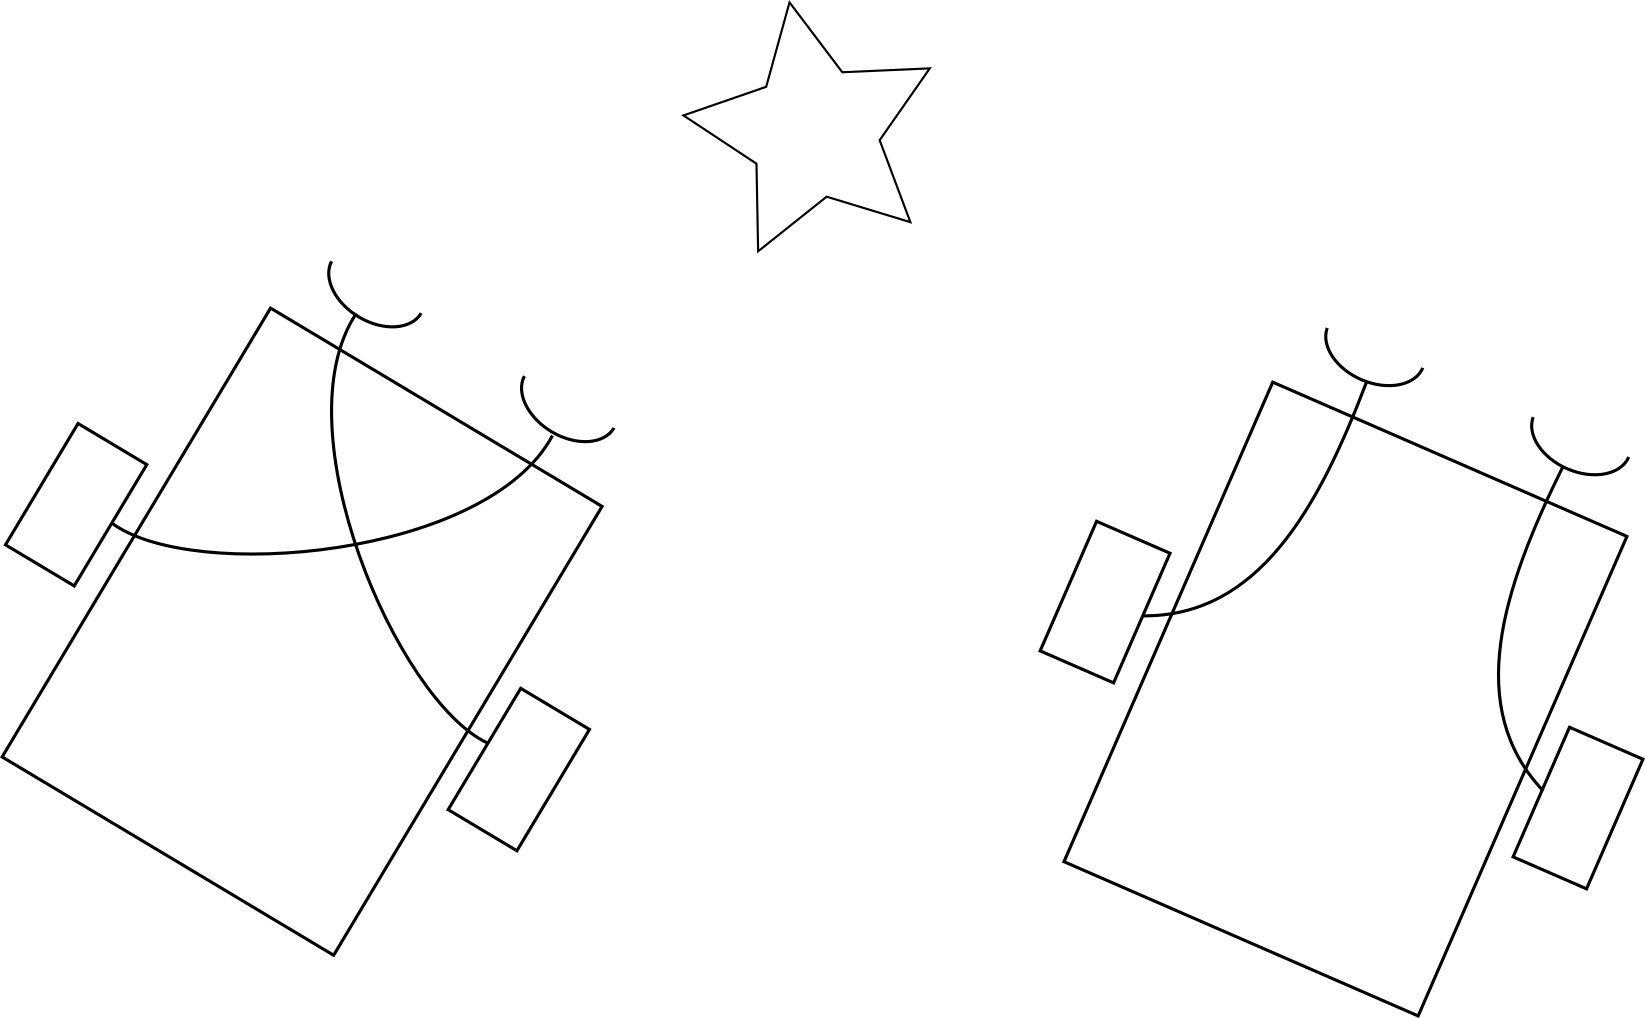
\includegraphics[width=0.7\columnwidth]{figs/braitenberg.png}
\caption{Two vehicles approaching a light source. The brighter the light, the more does each motor turn. The left vehicle will therefore approach the light by turning toward it, the right vehicle will avoid it by turning away from it.\label{fig:braitenberg}}
\end{figure}

A more complex behavior is obstacle avoidance. Assuming the output of an obstacle sensor to increase with the obstacle approaching (e.g., an infrared proximity sensor), we can use the same principle to compute the wheel speeds such that the obstacle is actively avoided. An example for a differential-wheel robot with eight infrared proximity sensors is given by
\begin{eqnarray}
\nonumber
\dot{\phi_l}&=&-6d_0-6d_1-19d_2-13d_3+94d_4+63d_5-50d_6-6d_7+b\\
\nonumber
\dot{\phi_r}&=&-6d_0+50d_1+63d_2+94d_3-22d_4-10d_5-6d_6-6d_7+b
\end{eqnarray}
%
% back, left {-0.06, -0.06}, 
% left {-0.06, 0.5}, 
% front, left {-0.19, 0.63}, 
% front, front, left{-0.13, 0.942}
% front, front, right {0.942, -0.22}, % left right motor
% front, right {0.63, -0.1}, 
% right {0.5, -0.06},  
% back, right {-0.06, -0.06},
%
with $d_0$ as the left rearward sensor and the other sensors being arranged clockwise such that $d_7$ is the right rearward sensing sensor, arranged as on the E-Puck differential wheel robot \cite{mondada2009puck}, see also Figure \ref{fig:epucksensors}.

\begin{figure}
\centering
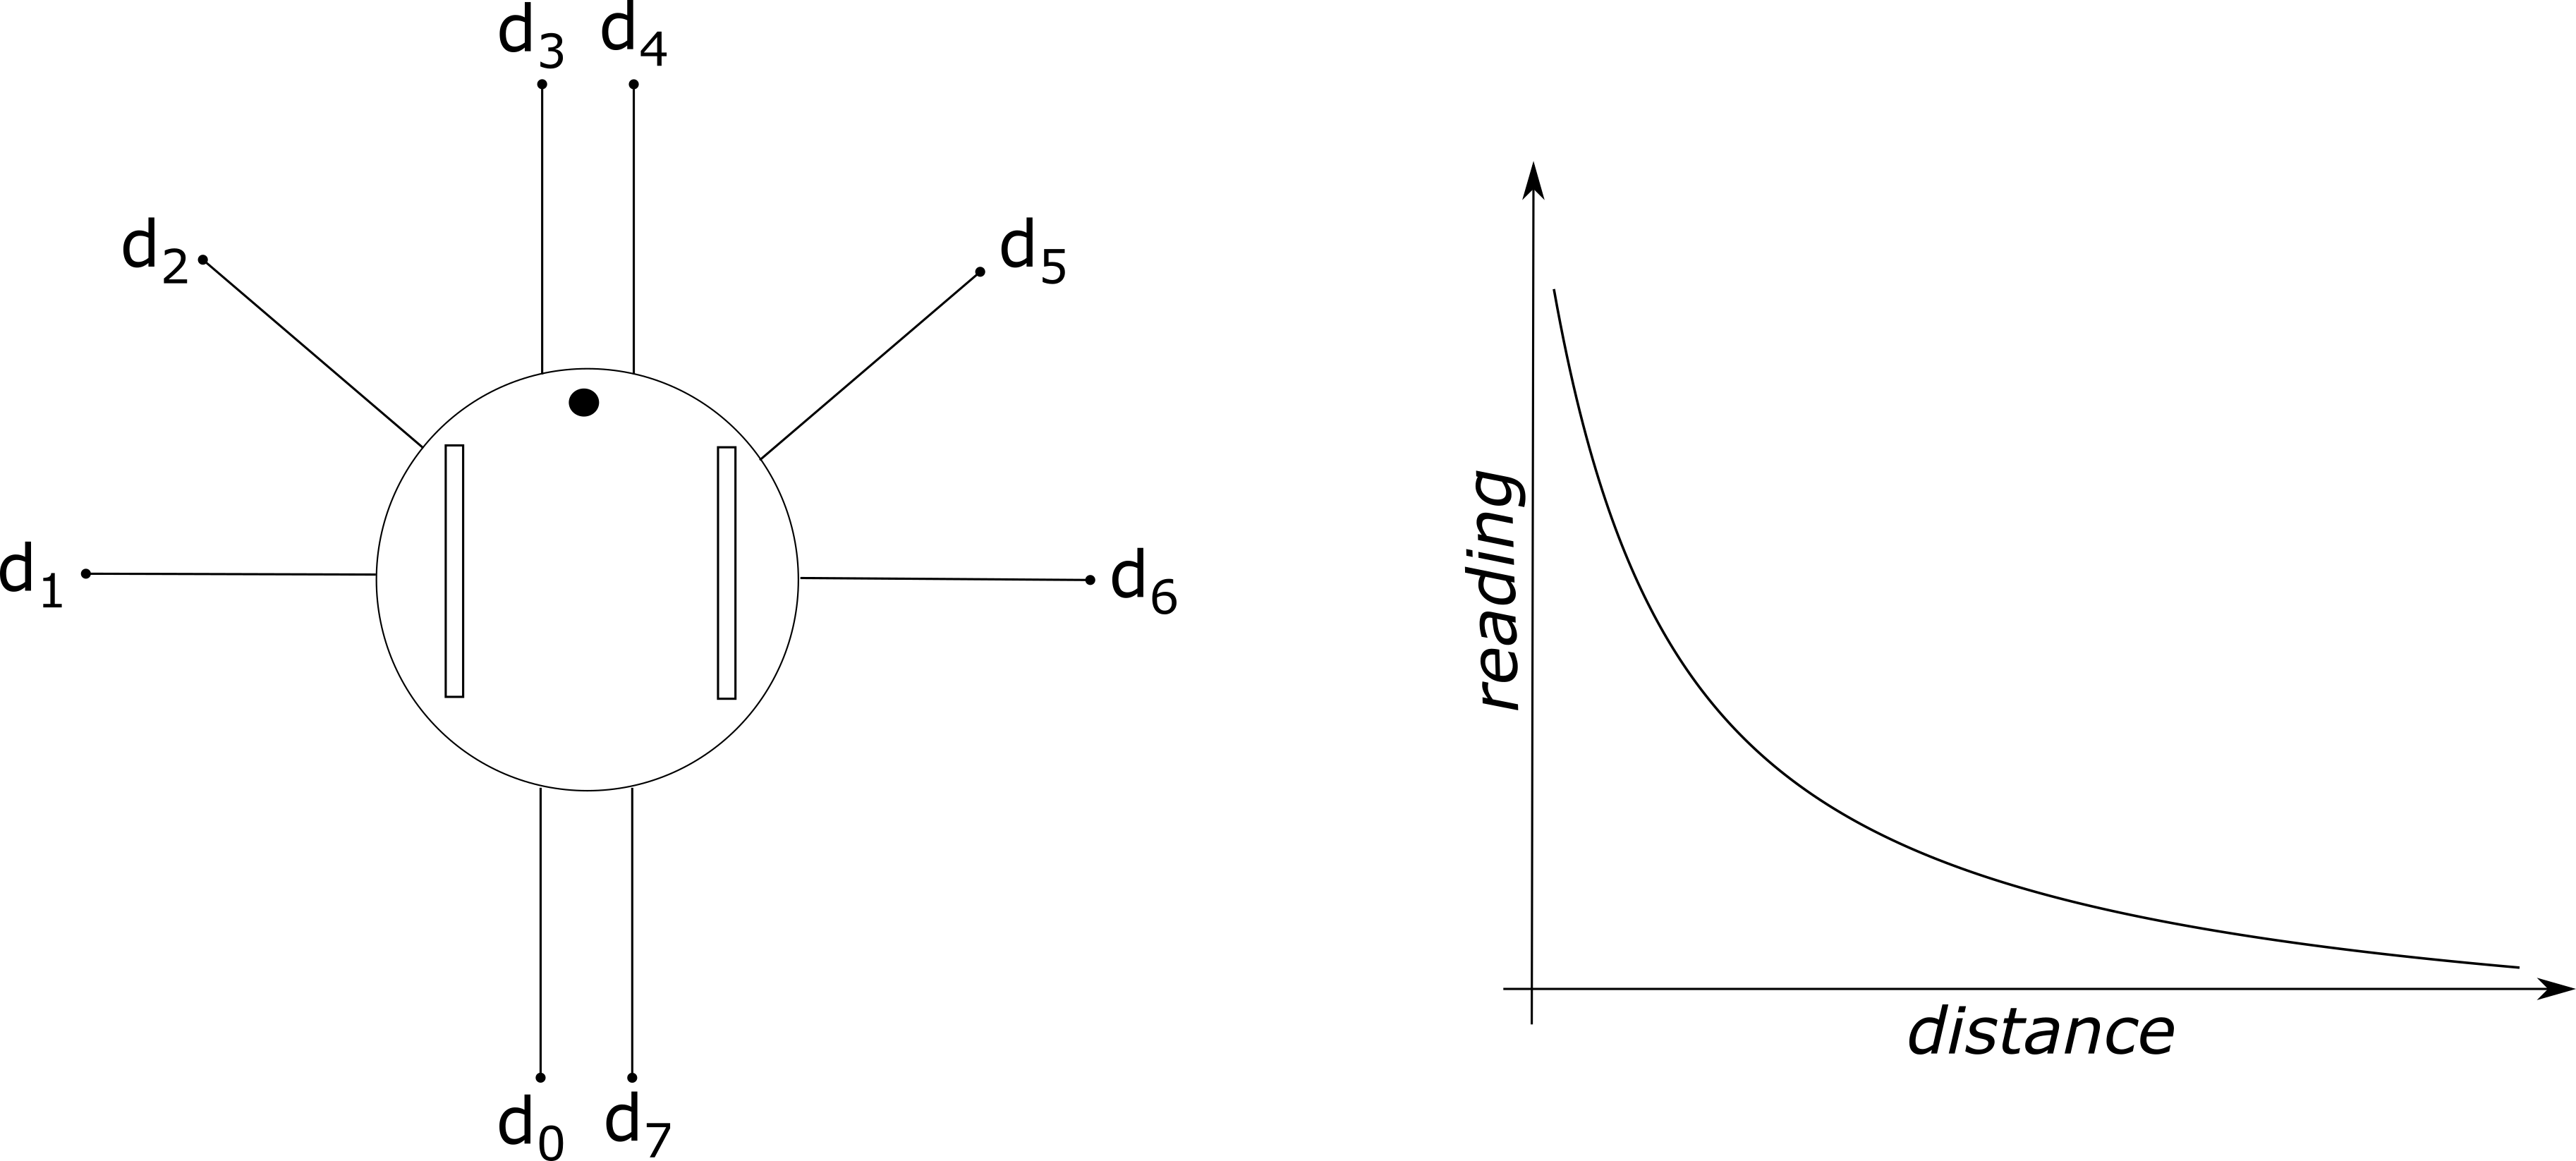
\includegraphics[width=0.9\columnwidth]{figs/ePuck.png}
\caption{\ref{fig:epucksensors}A schematic of a differential-wheel robot with eight infrared distance sensors (left) and typical sensor response as a function of distance (right).}
\end{figure}

Behaviors such as phototaxis and obstacle avoidance can also be combined by simply adding them and weighing each input accordingly. This idea has been popularized by the neuroscientist Valentino Braitenberg who augmented this system with additional ideas around learning (changing the weights based on events such as collisions), natural selection (building robots with random weights and selecting those that perform best), and analogies to the human brain \cite{braitenberg1986vehicles}. Controllers of these kind are therefore often called ``Braitenberg''.

Indeed, the controllers above bear strong resemblance to artificial neural networks such as described in Chapter \ref{chap:anns}, and ``optimal'' values to obtain a certain behavior can be obtained using evolutionary computation \cite{floreano1998evolutionary} or by training a neural network that yields appropriate input/output pairs. 

There are numerous variants of the control architecture including the \emph{subsumption architecture} \cite{brooks1990elephants} and \emph{motor schemas} \cite{arkin1989motor} that propose variations of switching different components of a reactive controller on and off to obtain desired behaviors. While useful for achieving relatively simple behaviors, these approaches are difficult to manage in practice and are better managed by being embedded in high-level control frameworks. 

\subsection{Limitations of reactive control}
The limitations of a reactive control scheme can be illustrated when considering that a robot combining both phototaxis and obstacle avoidance will still get stuck in a U-shaped obstacle. While obstacle avoidance will prevent the robot from hitting the obstacle, as soon as the way is clear, the robot will keep turning toward the light, thereby getting stuck in a loop. This type of behavior is also exhibited in simple insects such as flies or moths.

\begin{figure}
\centering
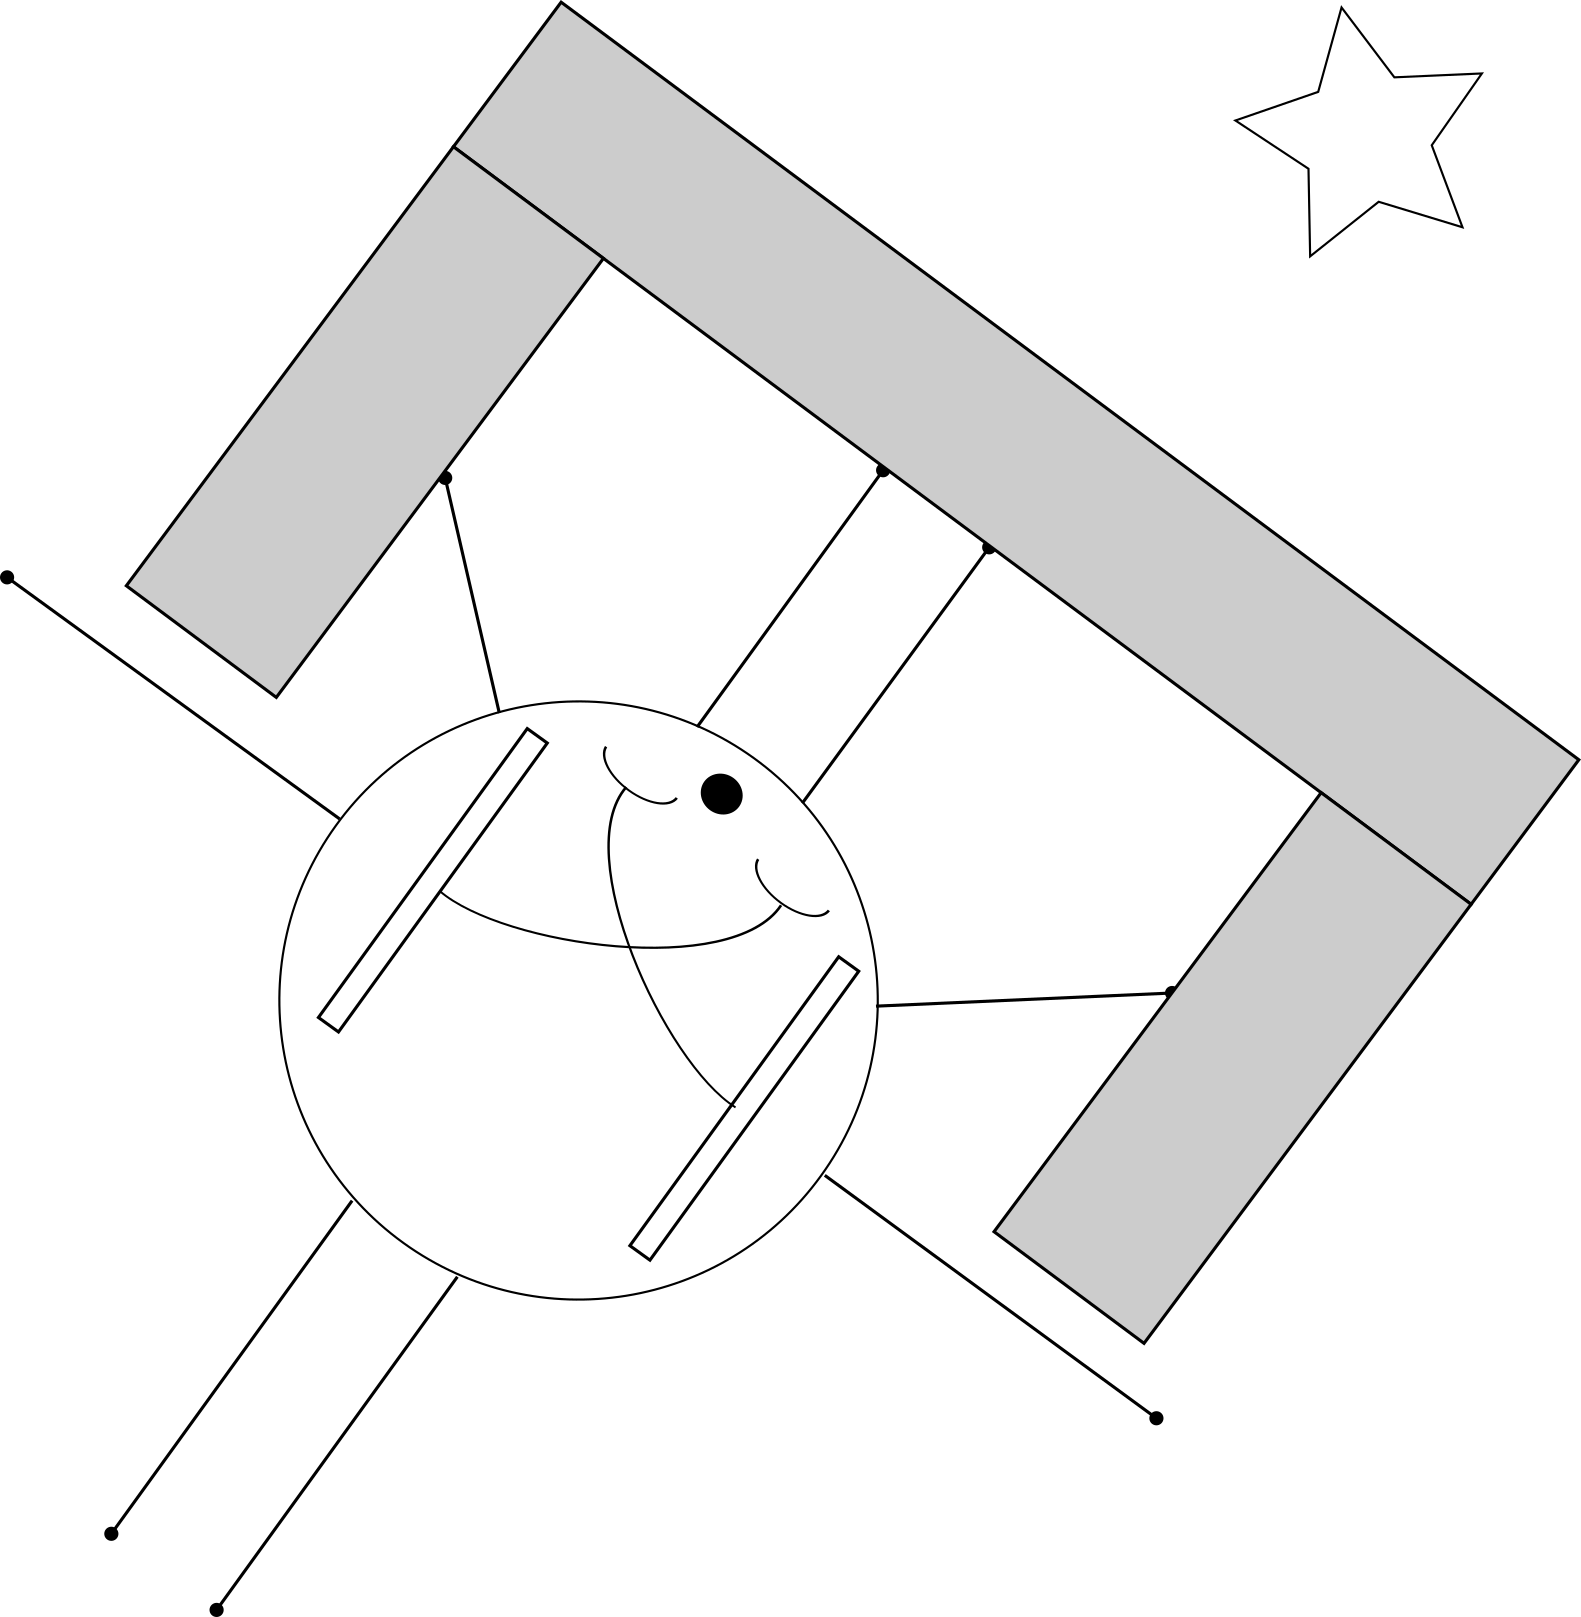
\includegraphics[width=0.8\columnwidth]{figs/uobstacle.png}
\caption{\label{fig:uobstacle}A differential wheel robot with distance and light sensors wired in a ``light following'' configuration in an U-shaped obstacle. Although the obstacle will be avoided, the light following behavior will continuously drive the robot into the obstacle unless state is added.}
\end{figure}


In order to avoid this situation, the robot needs to memorize its previous state and switch behaviors accordingly. For example, in addition to the basic combined avoidance and following behavior (``avoid and follow''), we can introduce an additional term (``wall following') in which the robot uses its proximity sensors to maintain a constant distance to a wall. In order to switch from one to the other behavior, we need to change the constant gains into dynamic ones that change their value based on other observations the robot makes. For example, the robot could estimate its progress by monitoring whether its light sensor is constantly increasing, and if it is not, inhibiting phototaxis behavior and emphasizing wall following. 

While feasible and potentially realizable with simple analog electronics, designing reactive systems with time-dependent behavior and state very quickly becomes difficult to manage. It is therefore desirable to establish discrete abstractions for various behaviors, which can be more easily managed and understood by a programmer. 
%
%
\section{Finite State Machines}\label{sec:fsm}
A simple, yet powerful tool to facilitate switching between different behaviors is a so-called \emph{Finite State Machine} (FSM)\index{Finite State Machine}\index{FSM}. In an FSM, each state is associated with a specific controller. In practice, an FSM consists of a global variable that stores the current state and a series of ``if'' statements that contain the code that is associated with each unique state. For example, an FSM to perform phototaxis while avoiding U-obstacles could consist of two states, with one for each desired behavior: one state that computes wheel-speeds so the robot moves toward the light while using its sensors to avoiding obstacles ahead of it, and another state that computes wheel-speeds so the performs a wall following behavior. To specify an FSM, one also needs to specify the \emph{state transitions}\index{state transition}\index{transition (state)}, the conditions that determine when to switch which state the FSM is in. For example, if multiple sensors detect an obstacle (implying that it may be a large one), then it may be desirable to have the FSM transition from its first state (phototaxis with simple obstacle avoidance) to its second (wall following). Finally, it is necessary to specify an initial state (the state the system starts in) and any final states (terminal states that signify program termination). An FSM can be depicted graphically, as shown in Figure \ref{fig:fsm_example}.

\todo{Insert FSM figure}
\begin{figure}
\caption{A simple Finite State Machine (FSM) with two states, an initial state, state transitions, and conditions that trigger a state transition.}
\end{figure}

Formally, a FSM is defined by a Tuple $(\Sigma, S, s_0, \delta, F)$ where:
\begin{itemize}
\item $\Sigma$ is the input \emph{Alphabet}, a set of symbols that represent events that can trigger state transitions,
\item $S$ is a finite set of states,
\item $s_0$ is an initial state, an element of $S$, that is $s_i \in S$,
\item $\delta$ is the state-transition function $\delta: S \times \Sigma \rightarrow S$ that maps combinations of states in $S$ and symbols $x$ in $\Sigma$ to a new state in $S$, and
\item $F$ is the set of final states, a subset of $S$. 
\end{itemize}

Historically, this definition stems from FSMs formally defining the working of a computer with a stream of symbolic commands of an actual program. In robotics, symbols that trigger state transitions can themselves be the result of complex computations. For example, a robot might switch to wall-following if it has not made actual progress toward its goal in some time and resume phototaxis once it reached a position that is closer to the light than it was before. 

In conjunction with a controller for each state, an FSM is called a \emph{Hybrid System}\cite{van2000introduction} as it combines both discrete (the state) and continuous (the controller outputs) variables. 

\subsection{Implementation}
A low-level robot controller is usually implemented as a loop with fixed loop time, for example 100ms for slow moving differential-wheel robots and 1ms for dynamical systems such as drones. At each start of the loop, the controller reads all sensors, then branches into the part of the code that corresponds to its current state, processes sensor information and computes actuator output, and finally sends the control commands to the actuators. 

Unlike a computer program that can process information as fast as possible, the robot controller needs to wait until sensor information are actually available, and actuator commands are executed (i.e. that the robot has physically moved). As the robot keeps moving while computation is ongoing, it is important to run the main loop at a constant rate. As computation is usually much faster than the loop time, it might be necessary to use an internal clock to wait until the loop time is expired. 


%@book{van2000introduction,
%  title={An introduction to hybrid dynamical systems},
%  author={Van Der Schaft, Arjan J and Schumacher, Johannes Maria},
%  volume={251},
%  year={2000},
%  publisher={Springer London}
%}



\begin{enumerate}
\item State is kept by a global variable
\item Robot program is executed in a loop, switch statement is used to enter different branches
\item Each state includes conditionals that set next state
\item Loop execution time is constant, usually done via sleep statements. This is important as odometry computations require a constant time to function.
\item FSMs are difficult to maintain. Adding a state requires modifiying the transitions of all states leading into that state and possibly also out of that new state.
\end{enumerate}

\section{Hierarchical Finite State Machines}\label{sec:stateflow}
\begin{enumerate}
\item FSMs are grouped into clusters, creating super-states
\item Also known as ``Statecharts'' \cite{harel1987statecharts}

\item State transitions between super states can be tied to states in the included FSM or be implicitly connected to all states of the included FSM, which allows leaving the super state from every state therein.
\item Super states can also be executed in parallel, providing events that lead to state transitions in other FSMs
\item Robot control software like ROS, LCM, or Yarp provide frameworks to implement asynchronous Hierarchical FSMs (HFSM), allowing super-states to subscribe to messages published by other super-states as well as directly triggering state transitions across different processes running in parallel in a service model.
\item HFSM solve some of the problems of FSMs by increasing modularity, simplifying programmability, but still have the problem that $N$ states can lead to $N^2$ state transitions, each of which need to be manually coded.
\end{enumerate}

\section{Behavior Trees}\label{sec:behaviortrees}
A Behavior Tree provides structure for hierarchically organizing the decision-making flow of a system. The leaves of a Behavior Tree are ``Action Nodes'' that can represent actual discrete behaviors, such as ``Close Gripper'' or ``Find Block''. The root and internal nodes of the Behavior Tree are made up of ``Utility Nodes" that guide the path of traversal through the tree. One powerful aspect of this abstraction is that Behavior Trees specifying complex behaviors, such as ``Navigate to Kitchen", can be encapsulated within a single node of another tree.

\subsection{Node Definition and Status}
In a traditional implementation, the nodes within a Behavior Tree can return any of three statuses when queried: ``Success", ``Failure", or ``Running". The incorporation of a ``Running" status allows the Behavior Tree to use behaviors that operate over longer time periods, such as a block picking behavior that persists over multiple control cycles of a robot's main processing loop, including time required to plan the end-effector's path, the time required to physically move the robot to the destination, and the time required to close the gripper. In this example, the node might return ``Failure" if any of the individual behaviors didn't work or if the end-effector didn't successfully grasp the block by the end of the behavior, and ``Success" otherwise. Thus, each node in the Behavior Tree needs a rigidly defined notion of ``Success" or ``Failure" that can be propagated throughout the Behavior Tree, informing which sequence of behaviors is executed to achieve the desired result.

Unlike the Finite State Machine formalism from before that didn't incorporate an explicit notion of time, the ``Running" status enables nodes to operate using the information that their child nodes may take variable amounts of time, with each discrete unit of time defined as a \emph{tick}. This design choice simplifies the specification of control flow, and dramatically reduces the number of explicit transitions that are needed to model a system. Suffice to say, for a robot with a 100ms control loop, many of the discrete behaviors that a programmer would be interested in (such as turning 180 degrees or moving forward one meter) are likely to require more than a single program cycle. 

Nodes may also be parameterized, allowing for information computed from one node to be passed on and used in a subsequent node. Consider building a Behavior Tree for sorting blocks on a table into bins by color: one way to organize this Behavior Tree is repeating the sequence of behaviors ``Find Block", ``Pick Block", ``Get Block Color", ``Place Block in Bin" until no blocks remain. In this case, the behaviors ``Get Block Color" and ``Place Block in Bin" are connected, since the color of the block will determine which bin it should be placed in. This potential for interaction between nodes enables the powerful expressivity of this tool.

\subsection{Node Types}
Within a Behavior Tree, nodes can generally be classified based on their connectivity (do they have children, and if so, how many?) and function (is this a utility node that determines control flow, or is it an action node executing the action itself?). The three primary node types are \emph{composite}, \emph{decorator}, and \emph{action}. 

\emph{Composite nodes} have one or more children and are responsible for regulating the control flow. Three important examples of composite nodes are the \emph{sequence node}, \emph{selector node}, and \emph{parallel node}. A sequence node executes each of its child nodes in order, returning ``Failure" if a single one fails and ``Success" after all have finished successfully. A selector node executes each of its child nodes in order, but returns ``Success" once a single child node succeeds, only returning ``Failure" if all child nodes have failed. Sequence nodes can be thought of as analogous to an \emph{AND} conditional statement, while selector nodes are similar to an \emph{OR} conditional statement. Parallel nodes have $N>1$ children and attempts to execute its child nodes in parallel, returning ``Success" if $M$ or more children succeed and failure if more than $(N-M)$ children fail.

\emph{Decorator nodes} have exactly one child node and perform transformations on its child node's outputs back to its parents. An example of a simple decorator node is the \emph{Inverter}, a node that inverts the return status of its child, effectively producing a \emph{NOT} operation: if the child node returns ``Success" then the decorator returns ``Failure", and vice versa. Another useful decorator node is one that returns ``Success" when its child returns a status of either ``Success" or ``Failure", allowing for the inclusion of action nodes where success is not critical for the behavior. Decorator nodes can also be designed to repeat the execution of its child, for instance until it returns a ``Success" status, until it returns a ``Failure" state, or endlessly (which is typically placed as the tree's root node to ensure continuous operation).

\emph{Action nodes} have zero child nodes, and represent the execution of a discrete behavior. These nodes can use input parameters, return output values, and generally have any amount of complexity that the designer desires to program within them. Crucially, an entire Behavior Tree can be treated as a single action node, allowing for the composition of multiple Behavior Trees to build arbitrarily complex behaviors!

\todo{Insert pick and place BT figure, describe below}

\subsection{Behavior Tree Execution}
For each unit of time (e.g., control cycle) that passes, a preorder tree traversal occurs where nodes are recursively visited and evaluated left-to-right, commonly described as propagating a ``tick" signal through the tree. In doing so, each parent node calls on its child nodes in order to retrieve their status. If a child node returns ``Success", the parent node will move on to its next child node. If a child node returns a status of ``Running" then the parent node will return ``Running" without moving on to the next child node unless it permits running multiple child nodes in parallel. If a child node returns a status of ``Failure", its behavior will depend on the type of node of the parent, for example returning ``Failure" if the parent is a sequence node or moving on to the next child node if it is a selector node.






\begin{figure}
    \centering
    \begin{forest}
    {for tree={%
        minimum height = 4ex, 
        minimum width = 4ex, 
        draw, 
        parent anchor=south, 
        child anchor=north, 
        align=center
        }
    }
        [{\scriptsize Tilt Insert}\\ $\longrightarrow^*$
            [\scriptsize Rotate\\ $\theta_{tilt}$]
            [\scriptsize Move to\\ \scriptsize Contact \normalsize $-Z$]
            [\scriptsize Rotate\\ $-\theta_{tilt}-\delta \theta$]
            [\scriptsize Rotate\\ $\delta \theta$]
            [\scriptsize Hand at\\ $Z_{insert}$, ellipse]
        ]
    \end{forest}
    \caption{Tilt Insert Skill BT. The sequence first ..., then moves downwards until contact is made, rotates ... }
    \label{BTtilt}
\end{figure}

\begin{enumerate}
\item Programs are organized into nodes, each implementing certain functionality.
\item A node can have sub-nodes, like leafs of a tree, that are sequentially executed.
\item Each node can be \emph{running}, \emph{failed}, or \emph{successful}.
\item Execution within a node is triggered by a so-called \emph{tick} received by its parent node.
\item Nodes report their state back to their parent node.
\item A parent node issues ticks to its child nodes one by another, only moving to the next of its child nodes once the last one has returned \emph{successful}. (Or when a single one returns successful: ``Any" vs. ``All" type node)
\item As long as a child node is returning \emph{running}, it continues to receive ticks.
\item If a node fails, this information can be processed by the parent node who either passes it up, or restart the sequence of child nodes.
\item Popular in video game AI, give Minecraft example
\end{enumerate}

\section{Mission Planning}\label{sec:strips}
So far, we have seen how reactive behaviors can be composed into more complex programs using Finite State Machines and Behavior trees. Although Behavior Trees facilitate dealing with the exploding number of possible state transitions by making them implicit, the programmer still needs to define the entire program flow. Consider again a pick-and-place task. This time, we will not simply grasp a new item in case the object falls out of the hand, but try to find it on the table and try to pick it up from there. In a further advanced version, we might also go on and search for the object on the floor if it cannot be find on the table. But why not even have the robot replace an object from a warehouse if it cannot be found, or even mail order a new version? Obviously, it is very cumbersome to foresee all these eventualities when programming a robot. We therefore need a framework to make it easier. This is mission planning.

An example of mission planning is described in \cite{saito2011semantic} where a robot is tasked to provide a sandwich. The robot initially moves to a fridge, opens it and looks for a sandwich there, and then decides to take the elevator to the sandwich store in the basement of the University of Tokyo's engineering tower. Here, the robot is not only piecing together behaviors as it goes, but also using what is known as ``semantic planning'' to select the right actions, exploiting data bases of common sense knowledge in textual form. How to represent such knowledge in an efficient and general manner is an active research topic in robotics and artificial intelligence and goes beyond the scope of this introductory book. Yet, we will describe the basic algorithms that will allow you to compose complex behaviors during run-time, thereby generating much more complex robot responses than could ever be accomplished using hand-coding.

\subsection{The General Problem Solver and STRIPS}
One of the first planning frameworks has been introduced in 1959 as ``General Problem Solver'' (GPS) \cite{newell1959report,}, an idea that was popularized, refined and actually demonstrated on real robots later on as the ``STanford Research Institute Problem Solver'' (STRIPS)\cite{fikes1971strips}. 

In STRIPS, a robotic problem is composed of:

\begin{enumerate}
\item A set of symbols that represent the \emph{initial state}
\item A set of symbols that represent the desired \emph{goal state}
\item A set of \emph{actions}, each with a set of \emph{preconditions} and a set of \emph{postconditions}. 
\end{enumerate} 

An action's preconditions are a set of symbols that need to be part of the current state for the action to execute. An action's postconditions is the set of symbols the action creates and thereby affect state. In a nutshell, a STRIPS planner will work backwards from a desired goal state, find actions that have equivalent post-conditions and then recursively try to satisfy these actions preconditions. 

Formally, an instance of a STRIPS problem is a quadruple $\langle P, O, I, G \rangle$:
\begin{itemize}
\item $P$ is a set of propositional variables that can be either true or false and exhaustively describe the world the robot operates in. 
\item $O$ is a set of operators, each itself a quadruple $\langle \alpha, \beta, \gamma, \delta \rangle$ whose entries determine the set of conditions that need to be true ($\alpha$) and that need to be false ($\beta$) for the action to take place, and a set of conditions that will be true ($\gamma$) and that will be false ($\delta$) if the action is successful. 
\item $I$ is a set of conditions $I \subset P$ that are initially true and define the initial state, all other conditions are initially false. 
\item $G$ is a tuple $\langle N, M\rangle$ in which $N$ is a set of conditions that need to be true and $M$ is a set of conditions that need to be false. 
\end{itemize}

\subsection{A classic example --- the hungry monkey}




\section{Exercises}

\begin{enumerate}
\item A differential wheel robot has three downward-facing light sensors at its tip. The sensors are spaced such that the robot can detect a black line on a white ground. Derive the equations for a line-following robot using the Braitenberg formalism.
\item Derive a control scheme that combines line following and obstacle avoidance. Discuss your choices assuming that the robot has to avoid obstacles at all cost. 
\item Use a robotic simulator of your choice to implement basic phototaxis and obstacle avoidance. 
\item Use a robotic simulator of your choice to implement basic wall-following behavior
\item Implement a simple finite state machine that combines obstacle avoidance, phototaxis and wall-following and is capable to escape from a U-shaped obstacle
\item A FSM implements the following behavior: perform photo-taxis until an obstacle is it; then perform wall-following for 10 time steps. Draw an appropriate Finite State Machine. How many states do you need?
\item A robot runs at a 100ms loop time. Performing sensor readings takes 3ms, odometry computations 15ms, and executing logic takes 30ms on average. Which of these operations is likely to fail if the task logic takes 80ms?
\item Formulate both a Finite State Machine and a Behavior tree for the game ``Rats Life'', label each state and conditional transition, and compare the two representations.
\end{enumerate}
